\documentclass[12pt,oneside]{amsart}

\title{Math 287 Homework 0}
\author{Andrew Moore}
\date{August 27, 2021} % the due date of the homework

\usepackage[T1]{fontenc}
\usepackage{amsmath,amsfonts,amssymb,amsthm}
\usepackage[letterpaper,margin=1.5in]{geometry}
\usepackage{graphicx} % for including pictures
\usepackage{hyperref} % for including hyperlinks


% Extra space between lines
\linespread{2.4}

\theoremstyle{remark}
\newtheorem{exer}{Exercise}

\newenvironment{answer}{\bigskip\noindent\emph{Answer.}}{\hfill$\diamond$\newline}

\begin{document}
\maketitle

\newpage
\begin{exer}
\begin{enumerate}
\item What is your "official" name as on the class roster?
\item What name do you like to go by in class?
\item How is your name pronounced?
\item What pronouns do you prefer (this could be she/her/hers, he/him/his, they/them/theirs, or other)?
\item What is something that you are excited to learn in this class?
\item What is something that you are concerned about in this class?
\item Is there anything else you would like me to know?
\end{enumerate}
\end{exer}

\begin{answer}
\begin{enumerate}
\item My "official" name is Andrew Moore.
\item Please call me Andrew.
\item It's pronounced \emph{"and-roo more"}.
\item I use he/him/his pronouns.
\item I'm excited to have a course to focus on the writing of mathematics.
\item I've been intimidated at times when encountering proofs in textbooks, and hope I can build confidence in reading and writing them.
\item I'm currently a non-degree student, but completed a BA in Psychology in 2013. I got involved with academic research under my advisor, and got really interested in statistics. I was intimidated by math in HS and early in college, but I've gained appreciation for the subject over time, and have enjoyed making up for lost time. My goal is to pursue a masters degree in applied math or stats. Assuming I do well in this course, I hope to join you in the spring for Real Analysis!
\end{enumerate}
\end{answer}

\newpage
\begin{exer}
Have you used \TeX~ or \LaTeX~ before?
\end{exer}

\begin{answer}
Sort of? I'm used to writing reports using RMarkdown. There's an R package called knitr that can compile markdown syntax into PDFs, and you can make use of LaTeX formatting/commands. I think this will be the first time I'll be making heavy use of equation formatting from LaTeX.
\end{answer}

\newpage
\begin{exer}
Simplify $(x+y)^2 - (x-y)^2$.
\end{exer}
\begin{answer}
$(x+y)^2 - (x-y)^2 = x^2 + 2xy + y^2 - (x^2 - 2xy + y^2) = 4xy$
\end{answer}

\newpage
\begin{exer}
Please share a math joke.
\end{exer}

\begin{answer}

A classic \href{https://xkcd.com/552/}{xkcd} comic. \newline

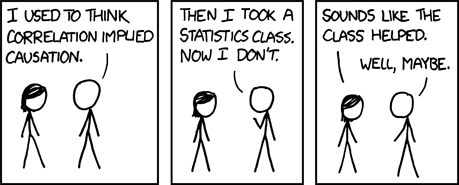
\includegraphics{../assets/correlation.png}

\end{answer}

\end{document}


